\section{Messung des Stillstandsdrehmomentes}

\subsection{Beschreibung}

Im zweiten Versuch soll der Ankwiderstand $R$ bestimmt werden.
Der Ankwiderstand kann über das Ohm'sche Gesetz berechnet werden, dafür ist
eine Matrix mit den Messwerten der Spannungen und Ströme gegeben.



\subsection{Ausgabe der Lösung}
\begin{figure}[htp]
 \centering
 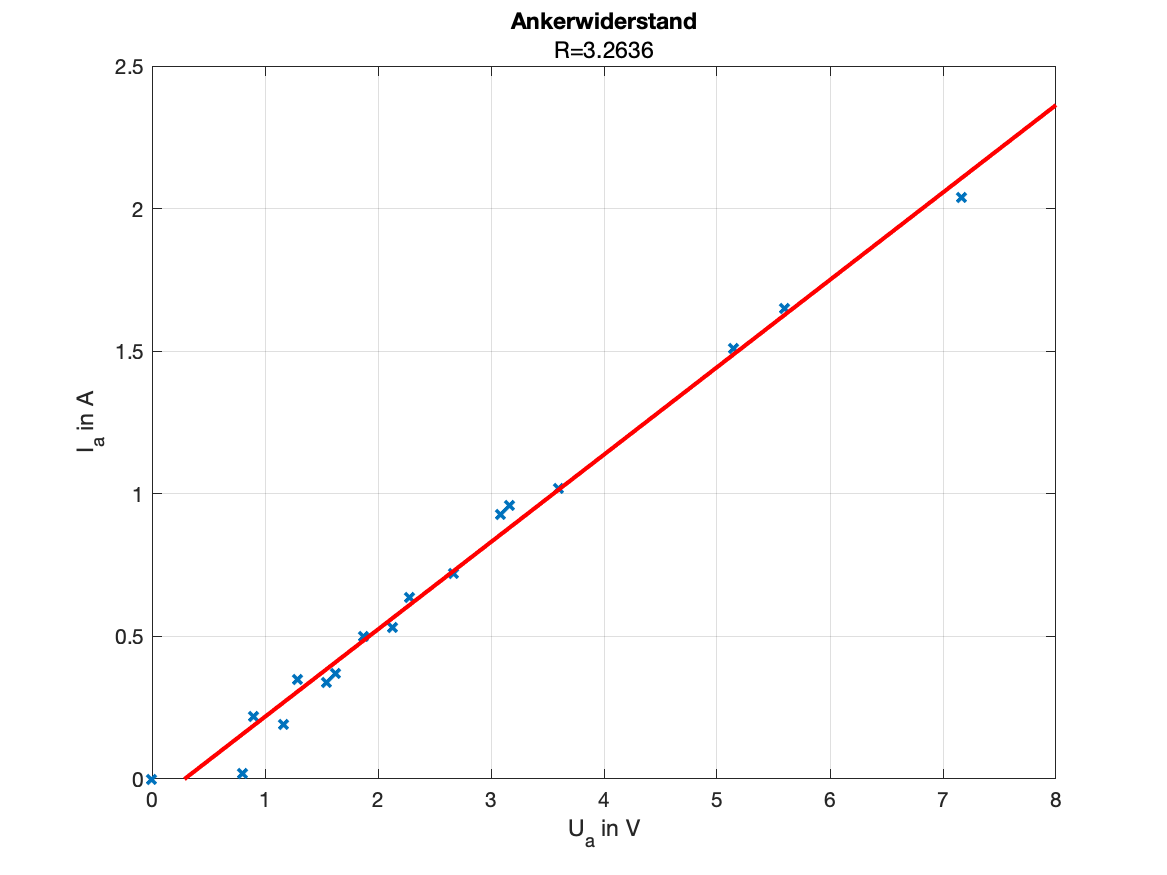
\includegraphics[width=1\textwidth]{as_labor01_2.png}
 \caption{Plot der Aufgabe 2}
 \label{fig:PlotAufgabe2}
\end{figure}

\subsection{Matlab Code}
\lstinputlisting[language=Matlab]{matlab/as_labor01_2.m}
